\scanpage{157}
On voit que c'est OK ssi $\forall x\in C$, l'application
\[
 \unsure{i_x|\iota_x}:u\longmapsto u_Cx,\qquad s^k\mathbin{\text{---}}C
\]
est dans $C\otimes_k s$, \deleted{\unsure{ssi}} i.e. (\unsure{en termes} d'une base $(e_\alpha)_{\alpha\in A}$ de $s$) se met sous la forme
\[
 u_Cx=\left(\sum_{\substack{\text{somme finie}\\x_\alpha\in C}}x_\alpha\otimes e_\alpha\right)(u)
 =\sum u(e_\alpha)x_\alpha
\]
ou encore, en posant
\[
 u(e_\alpha)=u_\alpha\qquad\text{donc }u\longmapsto(u_\alpha)_{\alpha\in A}\qquad s^k\simeq k^A
\]
\[
 u.x=\sum u_\alpha x_\alpha.
\]
\figure{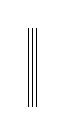
\begin{tikzpicture}\draw (0,0)--(0,1);\draw (.05,0)--(.05,1);\draw (.10,0)--(.10,1);\end{tikzpicture}}
Cela signifie aussi que $u\longmapsto u.x$ est continue pour la top. discrète sur $C$ et la top. de la convergence simple sur $s^k$.

Ou encore que
\[
 s^k\mathbin{\text{---}}\operatorname{Hom}_k(C,C)
\]
est continue, \unsure{qd} on met des deux côtés la top. de la conv. simple-discrète\ldots
\figure{\begin{tikzpicture}\draw (0,0)--(1,.2);\end{tikzpicture}}
Supposons maintenant que $s$\inserted{$=\sum s_n$} soit gradué
(pour $\Delta$) donc $s^k$ gradué,
\diagram{\begin{tikzcd}
s^k=\displaystyle\prod_{n\in D}s_n^k\arrow[r,phantom,"=" description]\arrow[r,bend right=35,"\mathrm{dfn}"'] & \displaystyle\prod_{n\in D}(s^k)_n.
\end{tikzcd}}
Soit $C$\inserted{$=\sum_{n\in D}C_n$} comodule gradué --- donc
\inserted{$C^k=\prod(C_n)^k=\prod(C^k)_n$}
\deleted{\unsure{co}}module gradué sur
\[
 s^k=\prod(s^k)_n=\prod(\unsure{C_n^k|s_n^k}).
\]
Alors \deleted{si $u\in s^k$ \unsure{$0$}} si $u\in(s^k)_n$,
\[
 (u_C)^k:\unsure{V(C_m^k)|C_m^k}\mathbin{\text{---}}\unsure{V(C_{m+n})|(C_{m+n})^k}
\]
donc
\[
 u_C:C_{m+n}\mathbin{\text{---}}C_m
\]
i.e. $u_C$ \uline{diminue} les degrés de $n$ ! (Pour qu'il les augmente il faut changer de signe les degrés de $C$ et plutôt exiger que
\[
 V(C)^m\overset{\mathrm{dfn}}=V(C_{-m})
\]
\unsure{---})
\margin{156}
